\chapter{Modelli e Funzionamento}\label{cap:modefunz}
\section{Blazor Server}\label{sez:bserver}
Il primo dei modelli ufficialmente rilasciati e per il quale si pu\'o ricevere supporto in produzione da settembre 2019\cite{blazorServerRelease}, \'e proprio questo.

Un'applicazione Blazor Server ospita i componenti Blazor lato Server e gestisce le interazioni dell'utente con la UI attraverso una connessione in tempo reale sfruttando SignalR.
Quando un utente scatena un evento, questo viene inviato attraverso la RTC al server, dove i vari componenti gestiscono l'evento.
Quando l'evento \'e stato gestito, blazor compara l'output generato con quello precedente l'evento, e manda quindi le sole differenze al browser del client, per poi applicarle al DOM.\cite{blazorModelsScenarios}

Blazor Server quindi necessita di una connessione stabile e a bassa latenza per funzionare al meglio, e gli scenari offline non sono supportati.

\'E particolarmente indicato quando si vuole delegare il costo computazionale al server e non ai client connessi, dato che ci\'o che il client esegue \'e il solo codice statico e le differenze di volta in volta inviate ma calcolate lato server.
Ci\'o rende molto veloce ed efficiente l'avvio dell'applicazione e in particolare il suo caricamento iniziale lato client, che rende il modello perfetto per funzionare su apparecchi a basso costo.

%Oltretutto ci\'o che viene scaricato lato client non varia al crescere dell'applicazione lato server.

\section{Blazor WebAssembly}\label{sez:bclient}
\section{Blazor PWA}\label{sez:bpwa}
\section{Blazor Hybrid}\label{sez:bhybrid}
\section{Blazor Native}\label{sez:bnative}
%\section{Stato Attuale delle Wireless Network}\label{sec:stato_attuale}
%
%Oggigiorno non esistono pi\`u dispositivi isolati che non comunicano con altri, tutti i PC prevedono la
%connessione ad internet, o in generale comunicano con altri dispositivi elettronici grazie alle reti di
%comunicazione. Inizialmente queste reti erano basate sui cavi ({\em wired network}), poi si sono rivelate
%pi\`u pratiche le reti senza filo ({\em wireless network}); da ci\`o si \`e dovuto affrontare il problema di
%permettere l'utilizzo delle tecnologie attualmente utilizzate nelle reti wired anche in reti wireless, che
%per loro natura sono intrinsecamente meno sicure a causa del mezzo trasmissivo. Le informazioni non vengono
%pi\`u convertite sotto forma di impulso elettronico e spedite su un filo metallico, ma essendo l'etere il
%mezzo di propagazione sono convertite in onde radio; queste ultime hanno una portata limitata non sempre ben
%determinabile, sono soggette a disturbi che degradano le informazioni inviate fino, a volte, a farle
%perdere; ed infine cosa a noi maggiormente sgradita l'energia consumata e direttamente connessa alla potenza
%trasmessa, ci\`o significa che aumentare la portata di trasmissione e la qualit\`a del segnale comporta un
%consumo maggiore dell'energia consumata.
%
%\section{Dynamic Power Management}\label{sec:dpm}
%
%Essendo la parte a radio frequenza colpevole del maggior consumo di energia, in particolare gli
%amplificatori utilizzati immediatamente prima dell'invio del segnale o dopo una ricezione, le stazioni
%802.11 possono allungare la vita delle batterie spegnendo i transceiver radio e mettendo la schada wireless
%in sleep periodicamente.
%
%Nella figura sottostante (Figura~\ref{fig:consumo_senza_ps}), si pu\`o osservare una finestra di 20~secondi
%del consumo di energia di una scheda wireless senza il power management abilitato:
%
%\begin{figure}[htbp]
%%\centerline{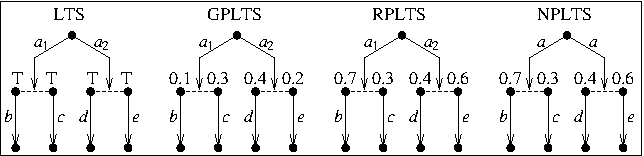
\includegraphics{figure/consumo_senza_ps}}
%%\caption{Consumo di energia senza power management}
%%\label{fig:consumo_senza_ps}
%\end{figure}
%
%Attivando il power management si pu\`o notare un sensibile risparmio energetico, a fronte di un diverso
%consumo energetico dovuto ad un diverso modo di operare: 
%
%\begin{figure}[htbp]
%%\centerline{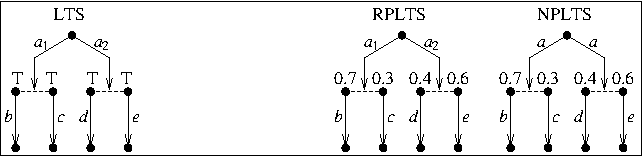
\includegraphics{figure/consumo_con_ps}}
%%\caption{Consumo di energia con power management}
%%\label{fig:consumo_con_ps}
%\end{figure}
%
%In questa modalit\`a la stazione resta per la maggior parte del tempo nello stato di sleep, risvegliandosi
%periodicamente (nella figura ogni 100~ms) per controllare se nel frattempo c'\`e stato traffico per essa.
%Durante il periodo di sleep, sar\`a demandato all'Access Point il compito di bufferizzare i frame destinati
%verso la scheda momentaneamente in sleep; al risveglio i frame bufferizzati saranno annunciati da un {\em
%Beacon frame}, la ricezione da parte della stazione wireless dei frame bufferizzati inizier\`a subito dopo
%con la loro richiesta tramite il {\em PS-Poll frame} (Figura~\ref{fig:power_saving}).
%
%\begin{figure}[htbp]
%%\centerline{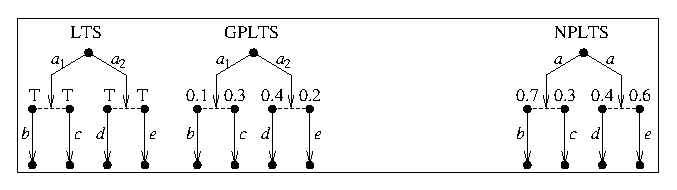
\includegraphics{figure/power_saving}}
%%\caption{Visione beacon e Ps-Poll}
%%\label{fig:power_saving}
%\end{figure}
%
%Quando viene attivato il power management l'Access Point e la stazione wireless devono sincronizzarsi per
%risvegliarsi ad intervalli prestabiliti, che nel caso della figura soprastante \`e 100~ms; all'inizio di
%ogni risveglio l'Access Point invier\`a il beacon contenente la {\em traffic indication map - TIM} che dice
%alla stazione se vi sono pacchetti bufferizzati destinati ad essa; in tal cosa la stazione risponder\`a con
%un PS-Pool contenente il suo Association ID. Grazie all'Association ID l'Access Point sar\`a in grado di
%selezionare i frame destinati alla stazione e provveder\`a ad inviarli.
